\documentclass{classrep}
\usepackage[utf8]{inputenc}
\usepackage{color}
\usepackage{graphicx}
\usepackage{float}

\studycycle{Informatyka, studia dzienne, I st.}
\coursesemester{VI}

\coursename{Komputerowe systemy rozpoznawania}
\courseyear{2018/2019}

\courseteacher{dr inż. Marcin Kacprowicz}
\coursegroup{poniedziałek, 14:10}

\author{
\studentinfo{Justyna Hubert}{210200} \and
\studentinfo{Karol Podlewski}{210294}
}

\title{Zadanie 1: Ekstrakcja cech, miary podobieństwa, klasyfikacja}
\svnurl{https://github.com/hubjust/KSR}

\begin{document}
\maketitle

\section{Cel}
Celem zadania było stworzenie aplikacji do klasyfikacji tekstów metodą k-NN, korzystając z różnych sposób ekstrakcji wektorów cech oraz istniejących miar podobieństwa porównać kategorie do tych przypisanych przez aplikację.

\section{Wprowadzenie}	

Zagadnieniem, jakim zajmowaliśmy się w ramach projektu jest klasyfikacja statystyczna, która jest rodzajem algorytmu statystycznego przydzielającego elementy do klas, bazując na cechach tych elementów. W ramach przeprowadzanego eksperymentu zaimplementowaliśmy klasyfikator k-najbliższych sąsiadów. \newline

Algorytm k najbliższych sąsiadów, nazywany także algorytmem k-nn, należy do grupy algorytmów leniwych, czyli takich, które nie tworzą wewnętrznej reprezentacji danych uczących, lecz szukają rozwiązania dopiero w momencie pojawienia się wzorca testującego. Przechowuje wszystkie wzorce uczące, względem których wyznacza odległość wzorca testowego [1]. Metoda k-nn wyznacza k sąsiadów, do których badany element ma najmniejszą odległość w danej metryce, a następnie wyznacza wynik w oparciu o najczęstszy element, wśród k najbliższych. W przypadku naszego projektu odległość definiujemy jako skalę podobieństwa tekstów. \newline

W ramach zadania zostały użyte 2 metody ekstrakcji cech: \newline

\begin{itemize}

\item Term frequency - metoda polegająca na zliczeniu częstości występowania danego słowa w dokumencie. Obliczana jest z poniższego wzoru:
$$
tf_{i,j}
= \frac{n_{i,j}}{\sum_{k}n{k,j}}
$$

\item Inverse document frequency - metoda polegająca na wyznaczeniu, czy dane słowo występuje powszechnie we wszystkich dokumentach. Jest to logarytmicznie skalowana odwrotna część dokumentów zawierających wybrane słowo (uzyskana poprzez podzielenie całkowitej liczby dokumentów przez liczbę dokumentów zawierających ten termin). Obliczana jest z poniższego wzoru:
$$
idf_{i}
= \log\frac{|D|}{|\{d : t_{i} \in d\}|}
$$
\newline
\end{itemize}

Do obliczenia odległości tekstów posłużyliśmy się 3 metrykami: \newline

\begin{itemize}
\item metryka Euklidesowa - w celu obliczenia odległości $ d_{e}(x,y) $ między dwoma punktami $ x, y $ należy obliczyć pierwiastek kwadratowy z sumy drugich potęg różnic wartości współrzędnych o tych samych indeksach, zgodnie ze wzorem:
$$
d_{e}(x,y)= \sqrt{ (y_{1} - x_{1})^2 + \cdots + (y_{n} - x_{n})^2 }
$$

\item metryka uliczna (Manhattan, miejska) - w celu obliczenia odległości $ d_{e}(x,y) $ między dwoma punktami $ x, y $ należy obliczyć sumę wartości bezwzględnych różnic współrzędnych punktów $ x $ oraz $ y $, zgodnie ze wzorem:
$$
d_{m}(x,y)= \sum_{k=1}^{n} | x_{k} - y_{k} |
$$

\item metryka Czebyszewa - w celu obliczenia odległości $ d_{e}(x,y) $ między dwoma punktami $ x, y $ należy obliczyć maksymalną wartość bezwzględnych różnic współrzędnych punktów $ x $ oraz $ y $, zgodnie ze wzorem:
$$
d_{ch}(x,y)= \max_{i} |x_{i} - y_{i}|
$$
\newline
\end{itemize}

\section{Opis implementacji}
Program został stworzony w języku C\#. Graficzny interfejs użytkownika został stworzony przy  wykorzystaniu Windows Presentation Foundation. Logika aplikacji została odseparowana od GUI, w zgodzie ze wzorcem projektowym Model-view-viewmodel (MVVM), poprzez implementacje trzech projektów (Logic, ViewModel i GUI).

% \newline TUTAJ JAKIS DIAGRAM UML \newline

\subsection{Logic}
Klasy Chebyshev, Euclidean oraz Manhattan odpowiadają za prawidłowe obliczenia odległości tekstów. Dziedziczą one z klasy abstrakcyjnej Metric. \newline

Klasa Article odwzorowuje artykuły wczytane do programu. Przechowuje informacje o dokumencie takie jak: tytuł, tekst, tagi, przypisane tagi, wektor cech, odległość. \newline

Klasa FeatureExtraction implementuje dwie metody ekstrakcji cech - term frequency oraz inverse document frequency. \newline

Klasa FileReader odpowiada za poprawne wczytywanie plików do programu - wyselekcjoowanie wybranych przez nas informacji (tytuł, teksy, przypisaną etykietkę) i na ich podstawie stworzenie obiektu klasy Article. Z wczytanego tekstu usuwane są słowa, które występują w wykorzystanej przez nas stop liście [2]. Ten zabieg ma za zadanie wykluczyć terminy, które nie wnoszą kluczowych, dla nas, informacji. Następnie, tekst zostaje poddane stemizacji, czyli usunięciu ze słowa końcówki fleksyjnej pozostawiając tylko rdzeń wyrazu. Do tego także wykorzystujemy zewnętrzną bibliotekę [3]. \newline

Klasa KnnAlgorithm odpowiada za implementację algorytmu k-najbliższych sąsiadów. W tym miejscu wyliczane są wystąpienia słów w podanych dokumentach. \newline

Klasa Sets odpowiedzialna jest za odpowiedni dobór danych testowych oraz treningowych. \newline

Klasa CategoryCompatibilityChecker ma za zadanie sprawdzić, czy dany artykuł zawiera jeden tag z danej kategorii, oraz czy ten tag zawiera się w tagach branych pod uwagę.

\subsection{ViewModel}
Projekt ViewModel ma za zadanie odseparować logikę programu od interfejsu graficznego. \newline

Klasa MainViewModel przyjmuje dane wejściowe od użytkownika i reaguje na jego poczynania wywołując wybrane akcje z logiki programu oraz odpowiada za odświeżanie widoków w interfejsie graficznym.  

\subsection{GUI}
Projekt GUI (graphical user interface) implementuje przejrzysty oraz łatwy w obsłudze graficzny interfejs użytkownika. 

\section{Materiały i metody}

Klasyfikacja tekstów została wykonana wszystkimi dostępnymi metodami ekstrakcji cech dla wszystkich trzech metryk. Dla każdego przypadku testowego dokonano klasyfikacji tekstu dla k $\in$ \{2, 3, 5, 7, 10, 15, 20\} najbliższych sąsiadów. Wyniki porównano z faktyczną etykietą danego artykułu. Za każdym razem zbiór treningowy stanowił 60\% artykułów, zaś zbiór testowy 40\%. \newline

Klasyfikacja dotycząca lokalizacji przeprowadzana była jedynie na danych, których pole places przyjmowało jedną z wartości: west-germany, usa, france, uk, canada, japan. \newline

Klasyfikacja dotycząca tematów przeprowadzana była jedynie na danych, które pole topics przyjmowało jedną z wartości: gold, cocoa, sugar, coffe, grain. \newline

Klasyfikacja własnych tesktów przeprowadzana była na danych, których pole author przyjmowało jedną z wartości: taylor swift, macklemore, twenty one pilots, eminem, ed sheeran, black eyed peas.

\section{Wyniki}

Wyniki dla kolejnych eksperymentów przedstawiają tabele. Tabele 1-3 przedstawiają odpowiednio eksperymenty przeprowadzone dla metryki Euklidesa, ulicznej oraz Czebyszewa przy użyciu Term frequency, natomiast Tabele 4-6 przedstawiają alogiczne dane dla Inverse document frequency. Zamieszczone wykresy mają za zadanie porównać jak dobrze radzą sobie metryki z daną kategorią.

\begin{table}[H]
	\centering
	\begin{tabular}{c c c c} 
		\hline
		\textbf{k} & \textbf{places [\%]} & \textbf{topics [\%]} &  \textbf{authors [\%]} \\ [0.5ex] 
		\hline
		\hline 
		2 & 74.4 & 53.7 & 39.0 \\ 
		3 & 78.5 & 52.2 & 43,9 \\
		5 & 80.2 & 52.2 & 48,8 \\
		7 & 81.0 & 53.7 & 36,6 \\
		10 & 81.5 & 60.4 & 36,6 \\
		15 & 81.6 & 62.7 & 39,0 \\
		20 & 81.4 & 61.2 & 36,6 \\ 
		\hline
	\end{tabular}
	\caption{Skuteczność klasyfikacji dla metryki Euklidesowej dla TF}
\end{table}

\begin{table}[H]
	\centering
	\begin{tabular}{c c c c} 
		\hline
		\textbf{k} & \textbf{places [\%]} & \textbf{topics [\%]} &  \textbf{authors [\%]} \\ [0.5ex] 
		\hline
		\hline 
		2 & 75.4 & 56.7 & 36,6 \\ 
		3 & 79.4 & 56.7 & 41,5 \\
		5 & 81.0 & 61.2 & 43,9 \\
		7 & 81.3 & 59.0 & 36,6 \\
		10 & 81.9 & 64.9 & 41,5 \\
		15 & 82.0 & 64.9 & 39,0 \\
		20 & 82.1 & 63.4 & 36,6 \\ 
		\hline
	\end{tabular}
	\caption{Skuteczność klasyfikacji dla metryki ulicznej dla TF}
\end{table}

\begin{table}[H]
	\centering
	\begin{tabular}{c c c c} 
		\hline
		\textbf{k} & \textbf{places [\%]} & \textbf{topics [\%]} &  \textbf{authors [\%]} \\ [0.5ex] 
		\hline
		\hline 
		2 & 80.3 & 14.9 & 17.1 \\ 
		3 & 80.3 & 44.0 & 17.1 \\
		5 & 80.3 & 44.0 & 17.1 \\
		7 & 80.3 & 44.0 & 17.1 \\
		10 & 80.3 & 44.0 & 17.1 \\
		15 & 80.3 & 44.0 & 17.1 \\
		20 & 80.3 & 44.0 & 17.1 \\ 
		\hline
	\end{tabular}
	\caption{Skuteczność klasyfikacji dla metryki Czebyszewa dla TF}
\end{table}

\begin{figure}[H]
	\centering
	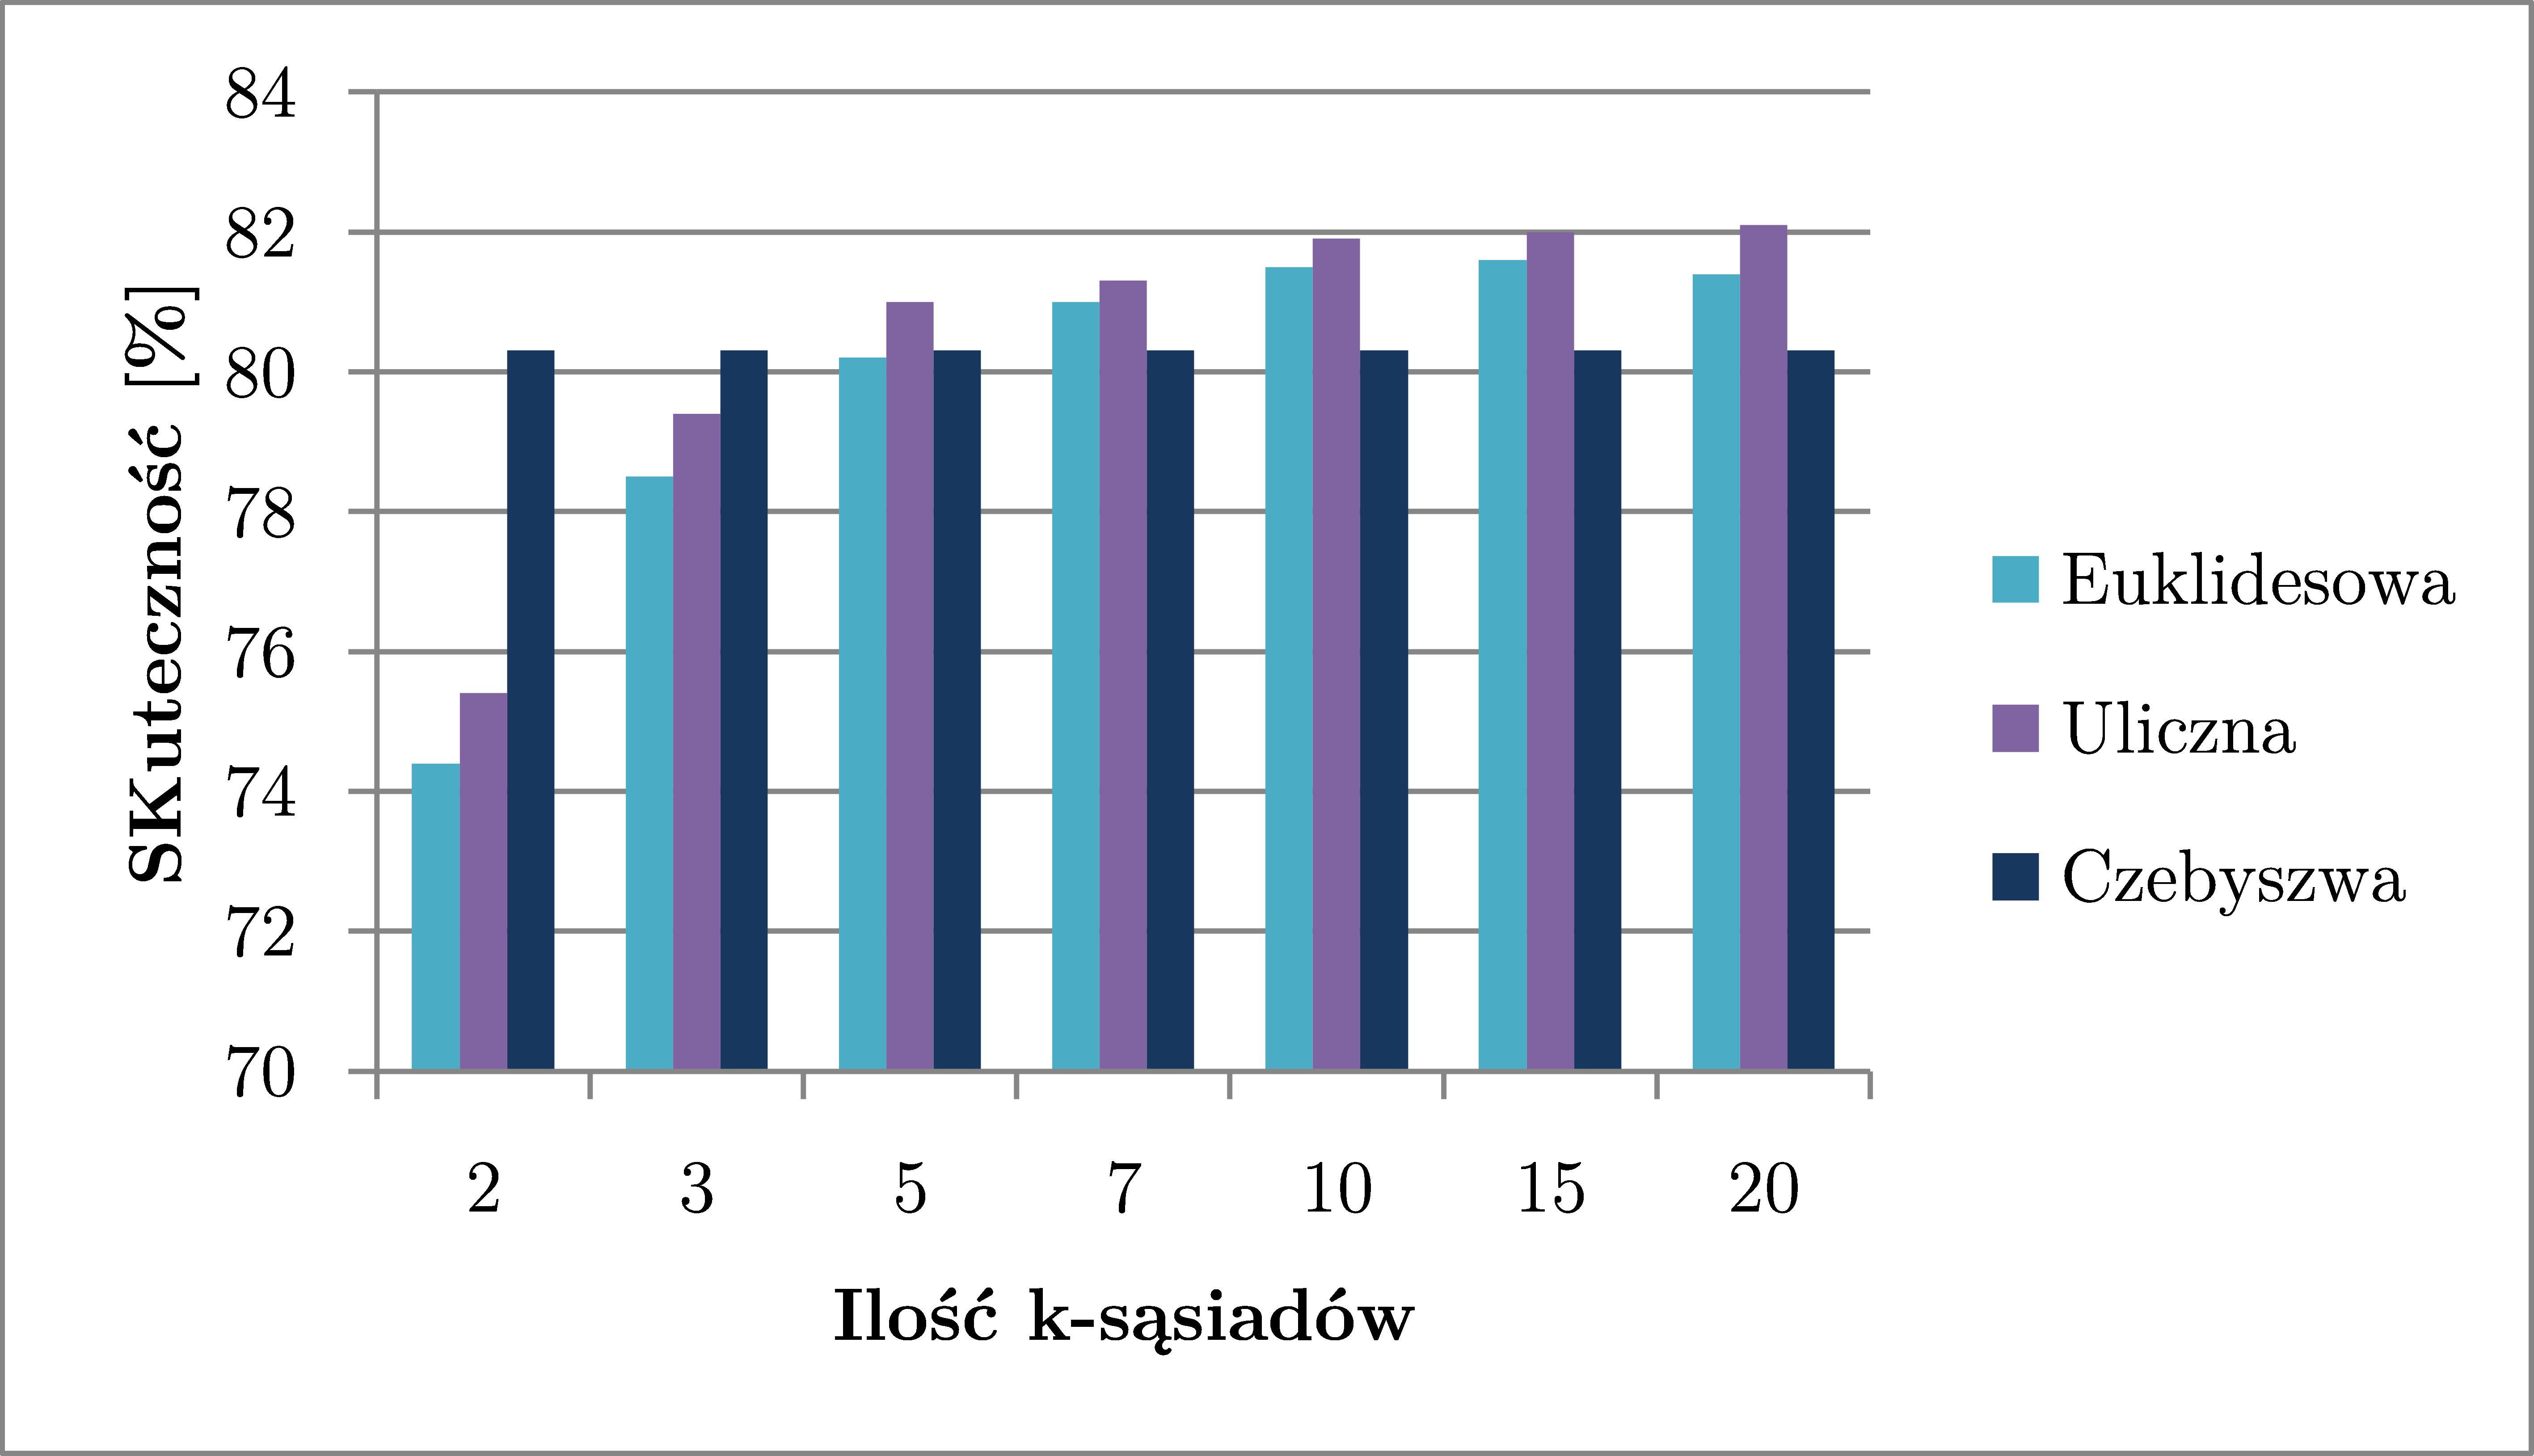
\includegraphics[width=0.8\textwidth]{{Rysunki/TF-places.png}}
	\caption{Dane z Tabel 1-3 dla kategorii places}
\end{figure}

\begin{figure}[H]
	\centering
	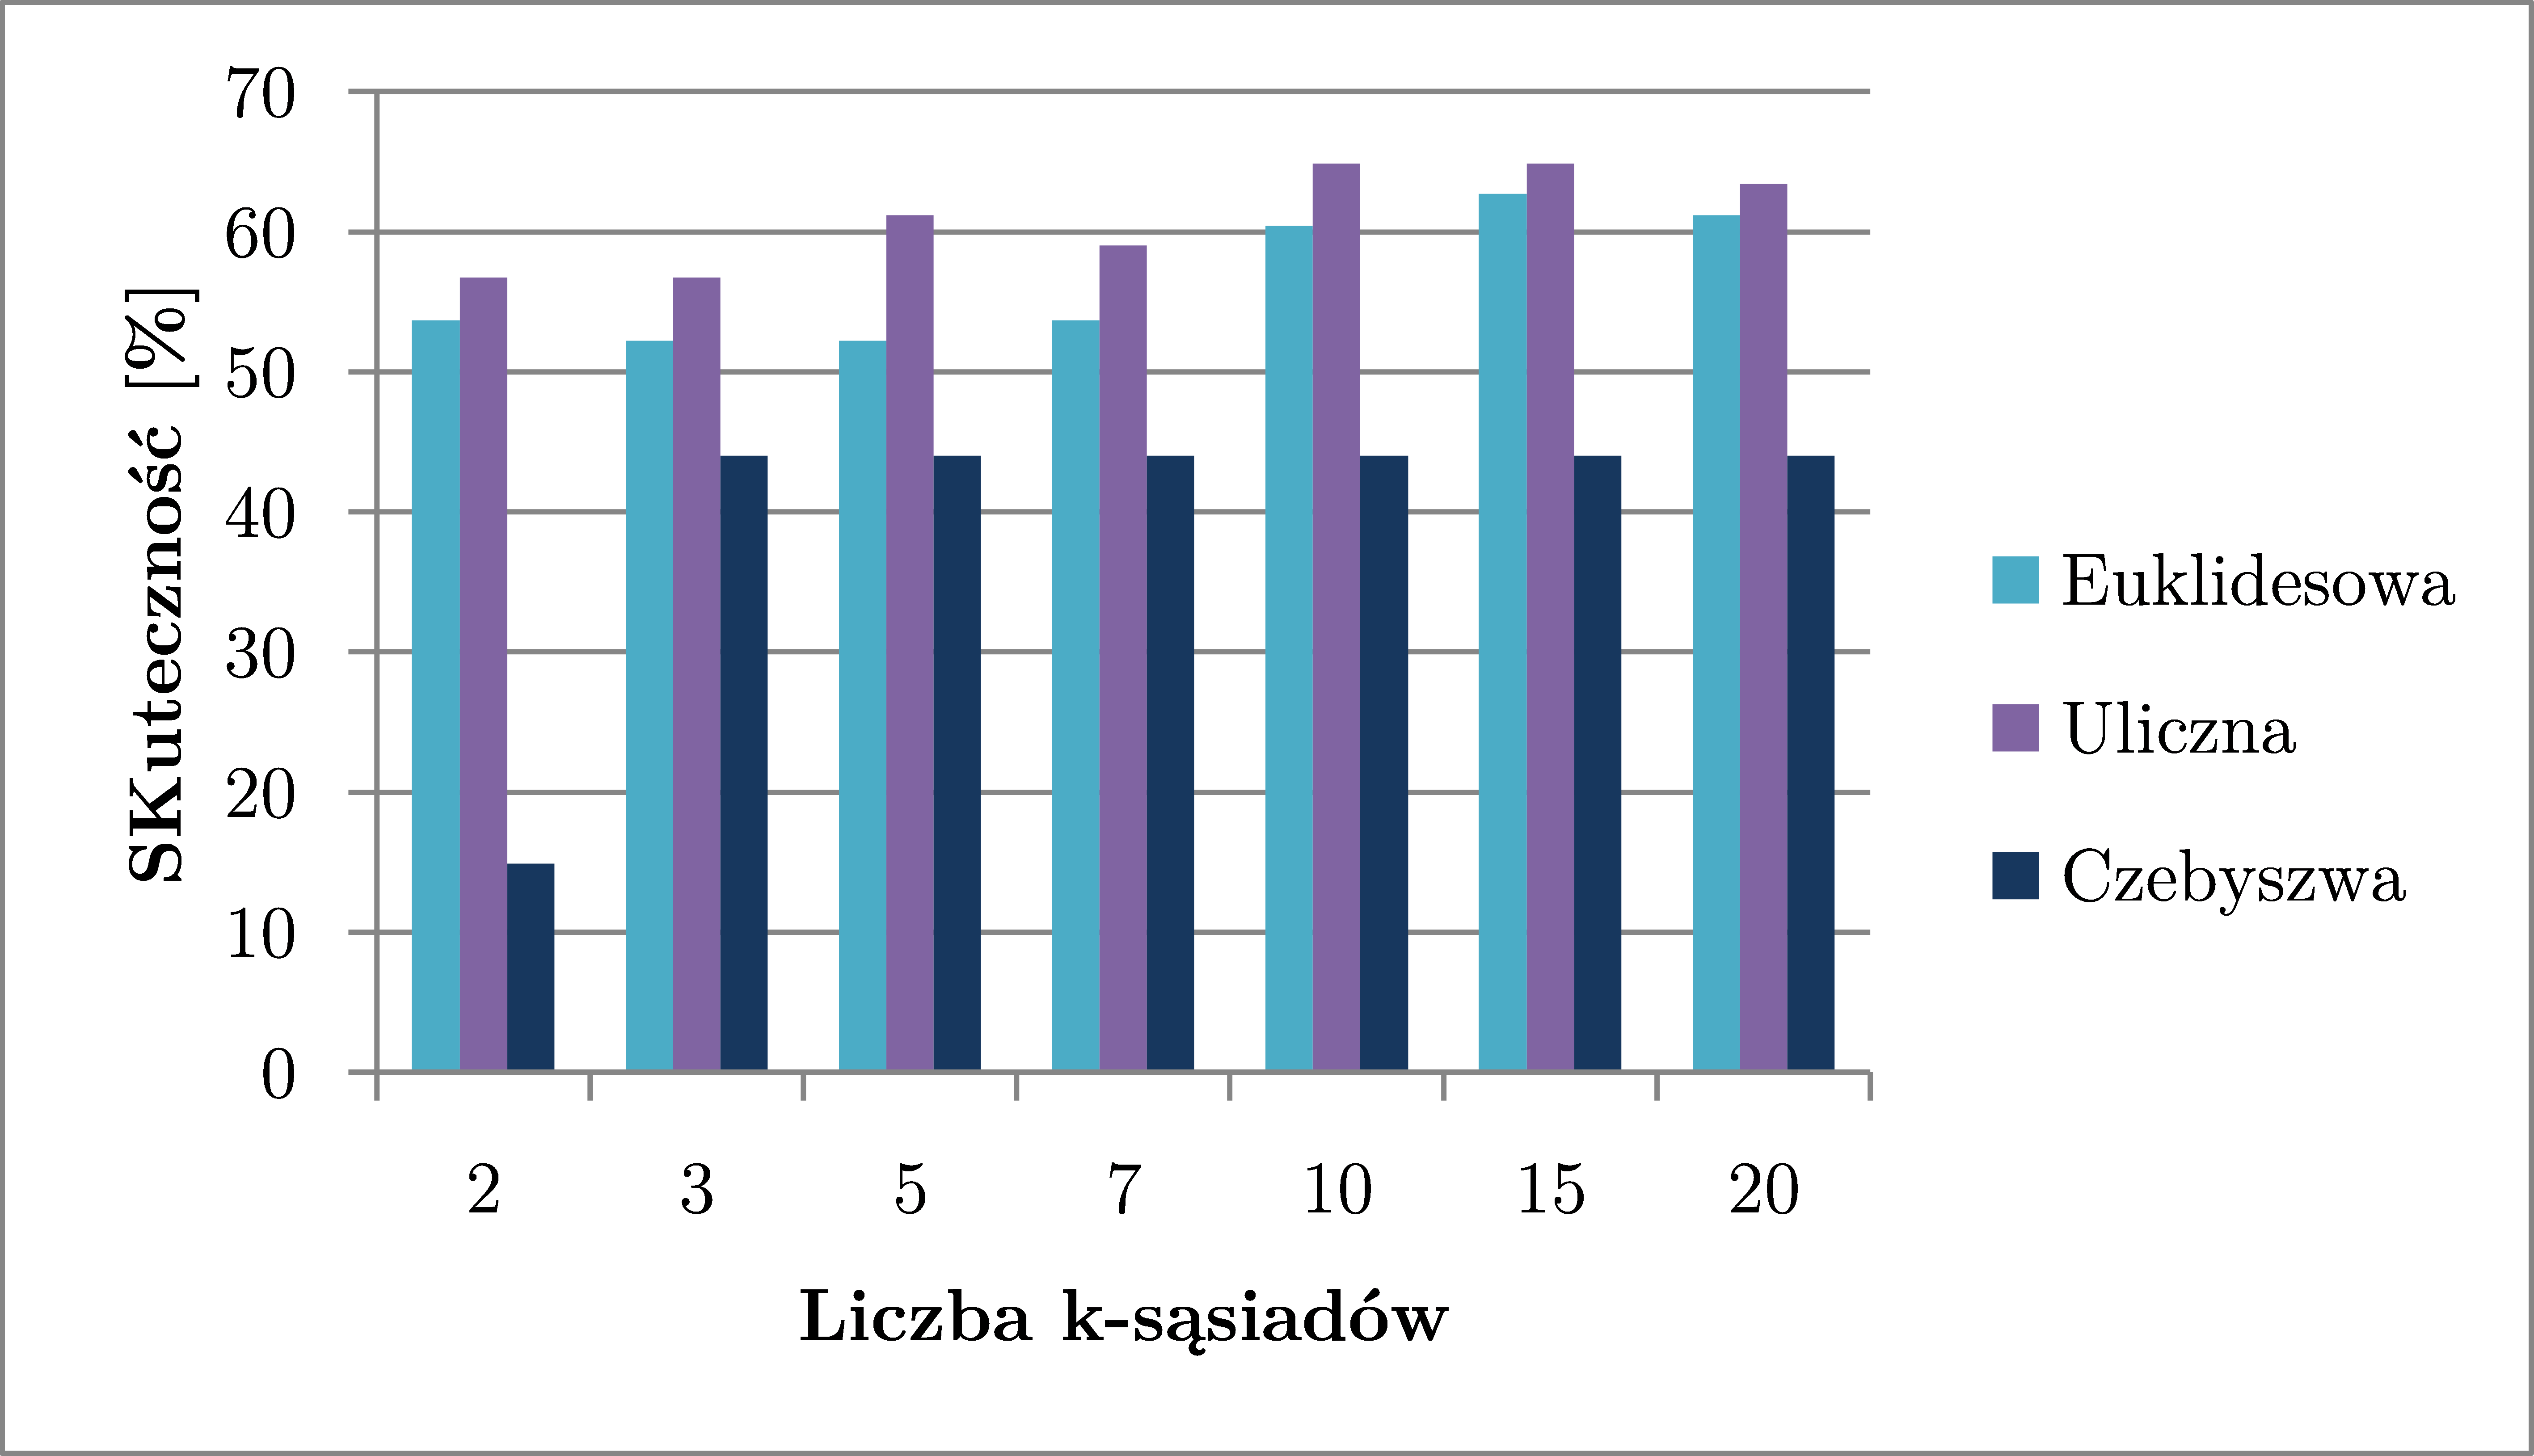
\includegraphics[width=0.8\textwidth]{{Rysunki/TF-topics.png}}
	\caption{Dane z Tabel 1-3 dla kategorii topics}
\end{figure}

\begin{figure}[H]
	\centering
	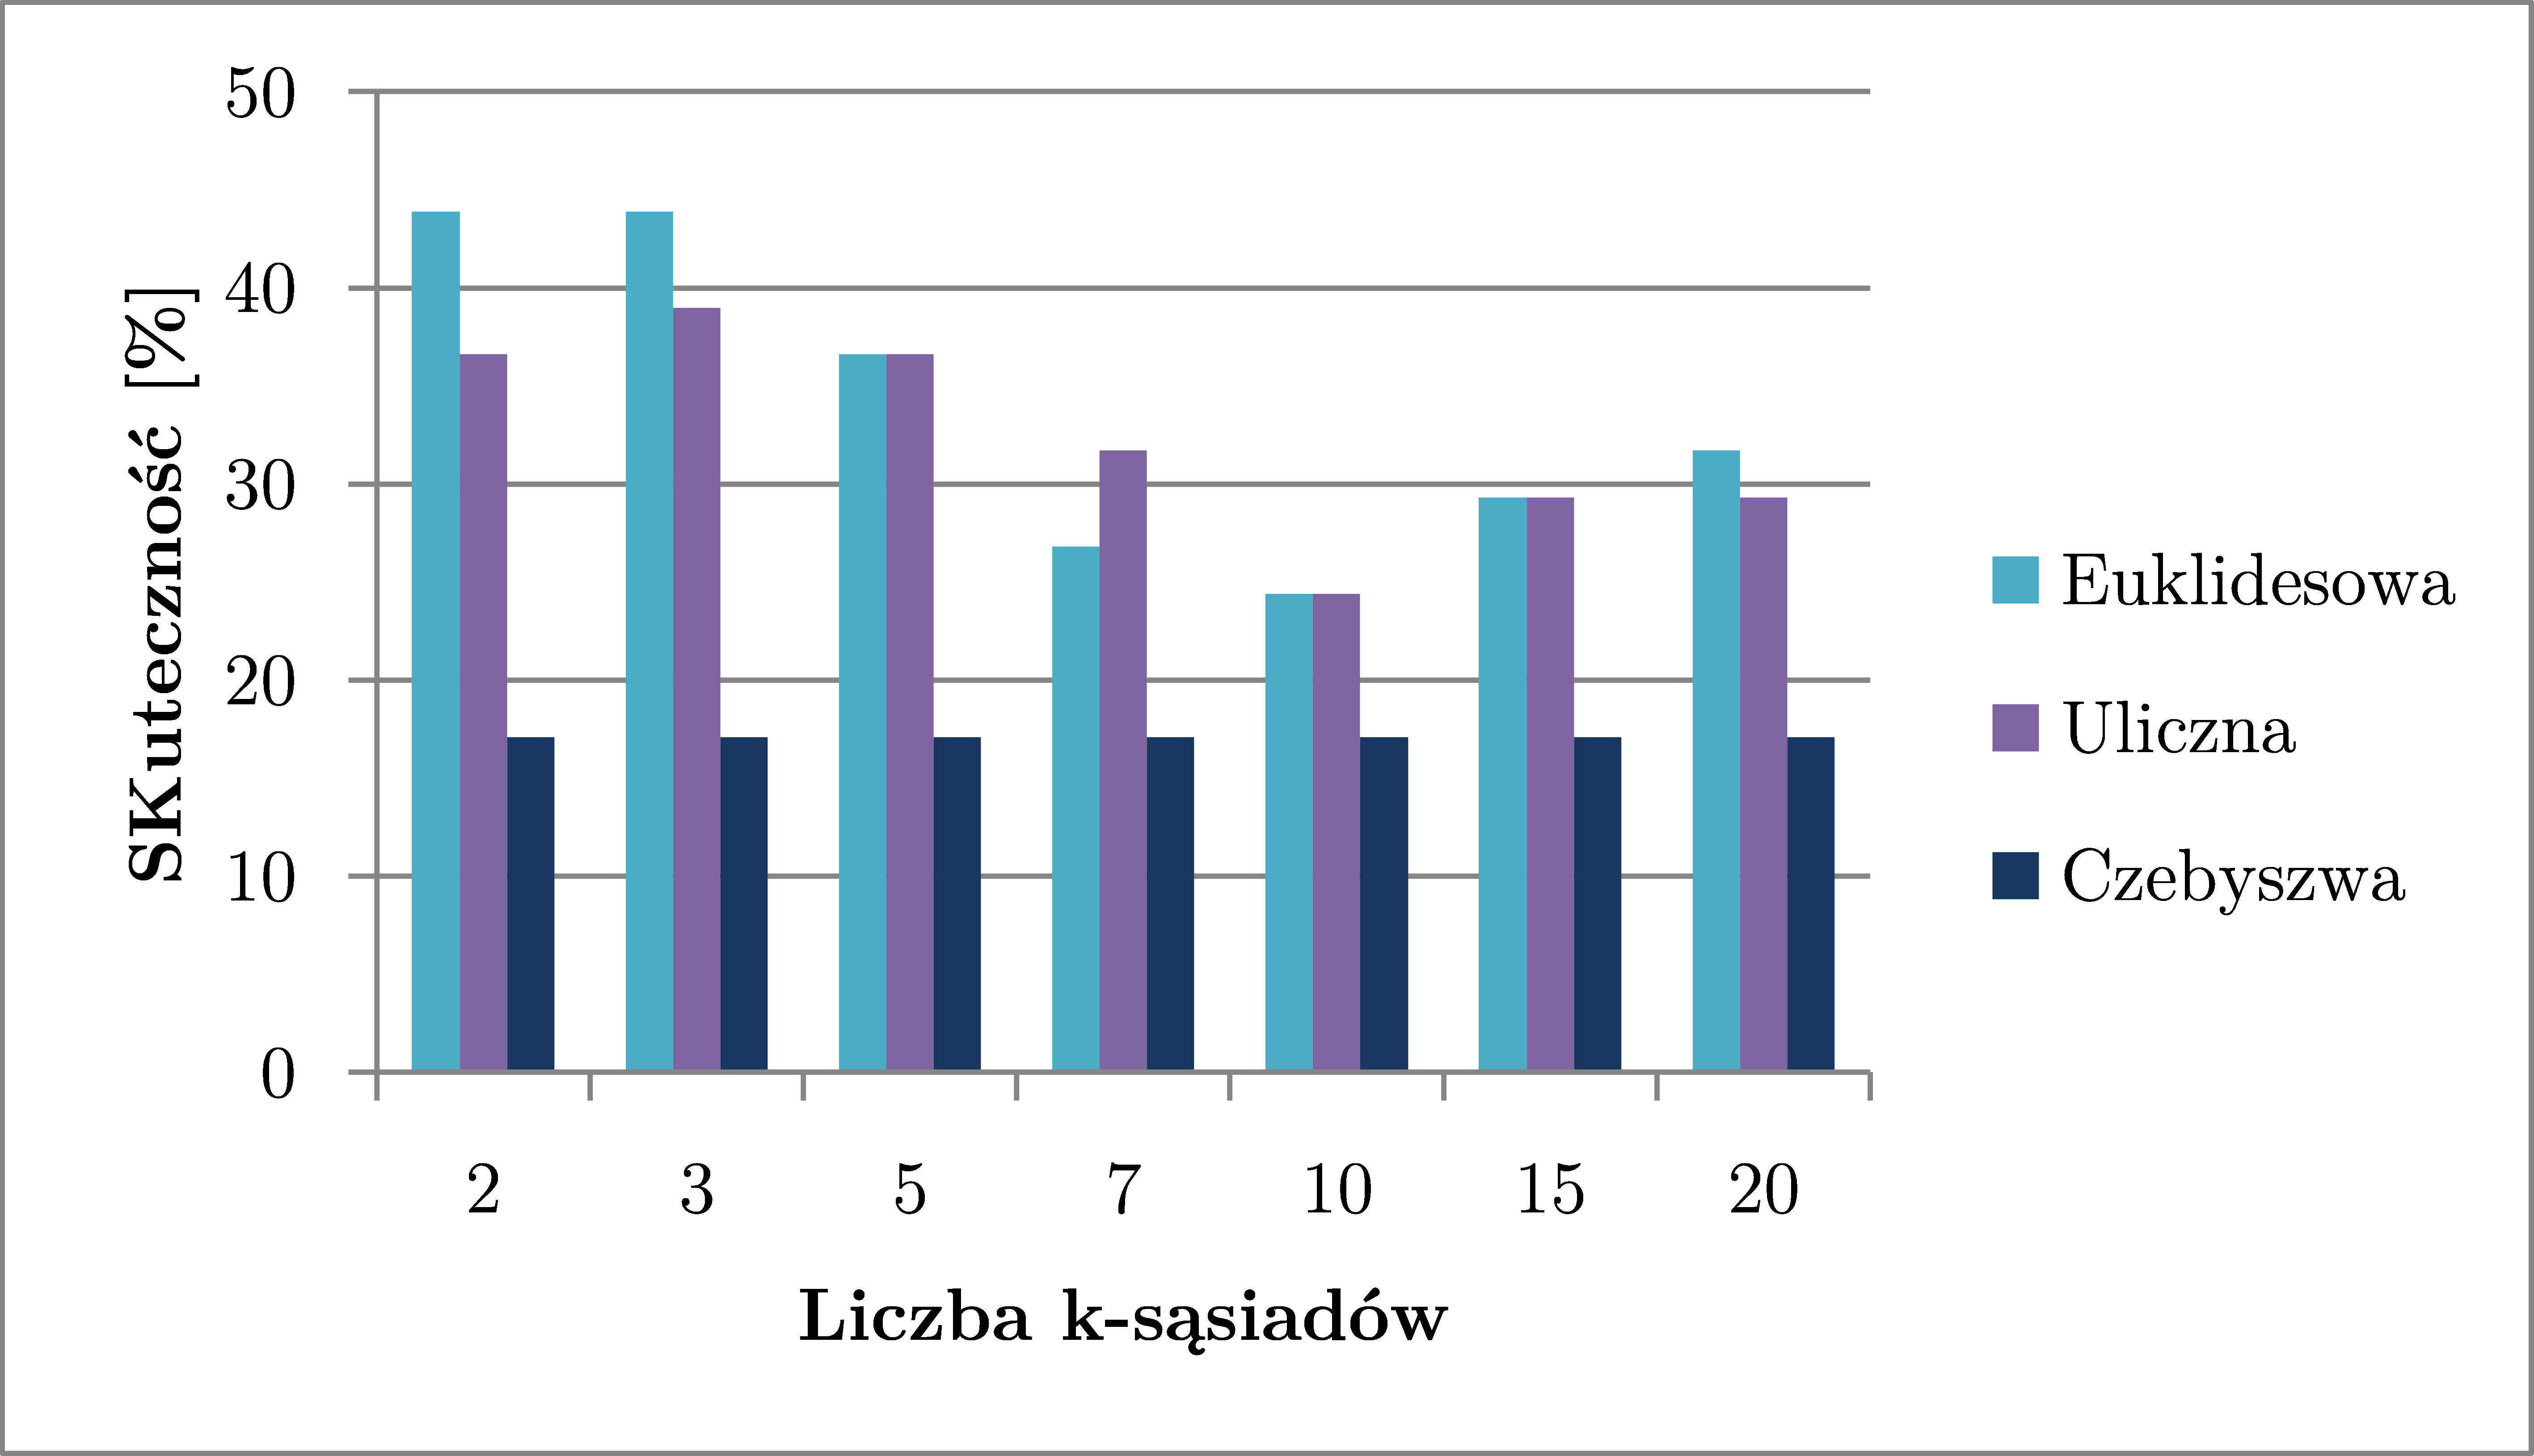
\includegraphics[width=0.8\textwidth]{{Rysunki/TF-authors.png}}
	\caption{Dane z Tabel 1-3 dla kategorii authors (własne teksty)}
\end{figure}

\begin{table}[H]
	\centering
	\begin{tabular}{c c c c} 
		\hline
		\textbf{k} & \textbf{places [\%]} & \textbf{topics [\%]} &  \textbf{authors [\%]} \\ [0.5ex] 
		\hline
		\hline 
		2 & 79,0 & 63,4 & 19,5 \\ 
		3 & 82,0 & 64,2 & 17,1 \\
		5 & 82,1 & 59,0  & 29,3 \\
		7 & 83,3 & 62,1 & 19,5 \\
		10 & 82,0 & 64,9 & 22,0 \\
		15 & 81,9 & 67,9 & 14,6 \\
		20 & 81.1 & 67,1 & 14,6 \\ 
		\hline
	\end{tabular}
	\caption{Skuteczność klasyfikacji dla metryki Euklidesowej dla IDF}
\end{table}

\begin{table}[H]
	\centering
	\begin{tabular}{c c c c} 
		\hline
		\textbf{k} & \textbf{places [\%]} & \textbf{topics [\%]} &  \textbf{authors [\%]} \\ [0.5ex] 
		\hline
		\hline 
		2 & 80,2 & 59,7 & 19,5 \\ 
		3 & 82,4 & 65,7 & 17,1 \\
		5 & 82,6 & 67,2 & 29,3 \\
		7 & 83,3 & 67,2 & 16,5 \\
		10 & 82,6 & 67,2 & 22.0 \\
		15 & 82,1 & 67,2 & 14,6 \\
		20 & 81,6 & 67,9 & 14,6 \\ 
		\hline
	\end{tabular}
	\caption{Skuteczność klasyfikacji dla metryki ulicznej dla IDF}
\end{table}

\begin{table}[H]
	\centering
	\begin{tabular}{c c c c} 
		\hline
		\textbf{k} & \textbf{places [\%]} & \textbf{topics [\%]} &  \textbf{authors [\%]} \\ [0.5ex] 
		\hline
		\hline 
		2 & 77.0 & 14.9 & 17.1 \\ 
		3 & 77.0 & 44.0 & 17.1 \\
		5 & 77.0 & 44.0 & 17.1 \\
		7 & 77.0 & 44.0 & 17.1 \\
		10 & 77.0 & 44.0 & 17.1 \\
		15 & 77.0 & 44.0 & 17.1 \\
		20 & 77.0 & 44.0 & 17.1 \\ 
		\hline
	\end{tabular}
	\caption{Skuteczność klasyfikacji dla metryki Czebyszewa dla IDF}
\end{table}

\begin{figure}[H]
	\centering
	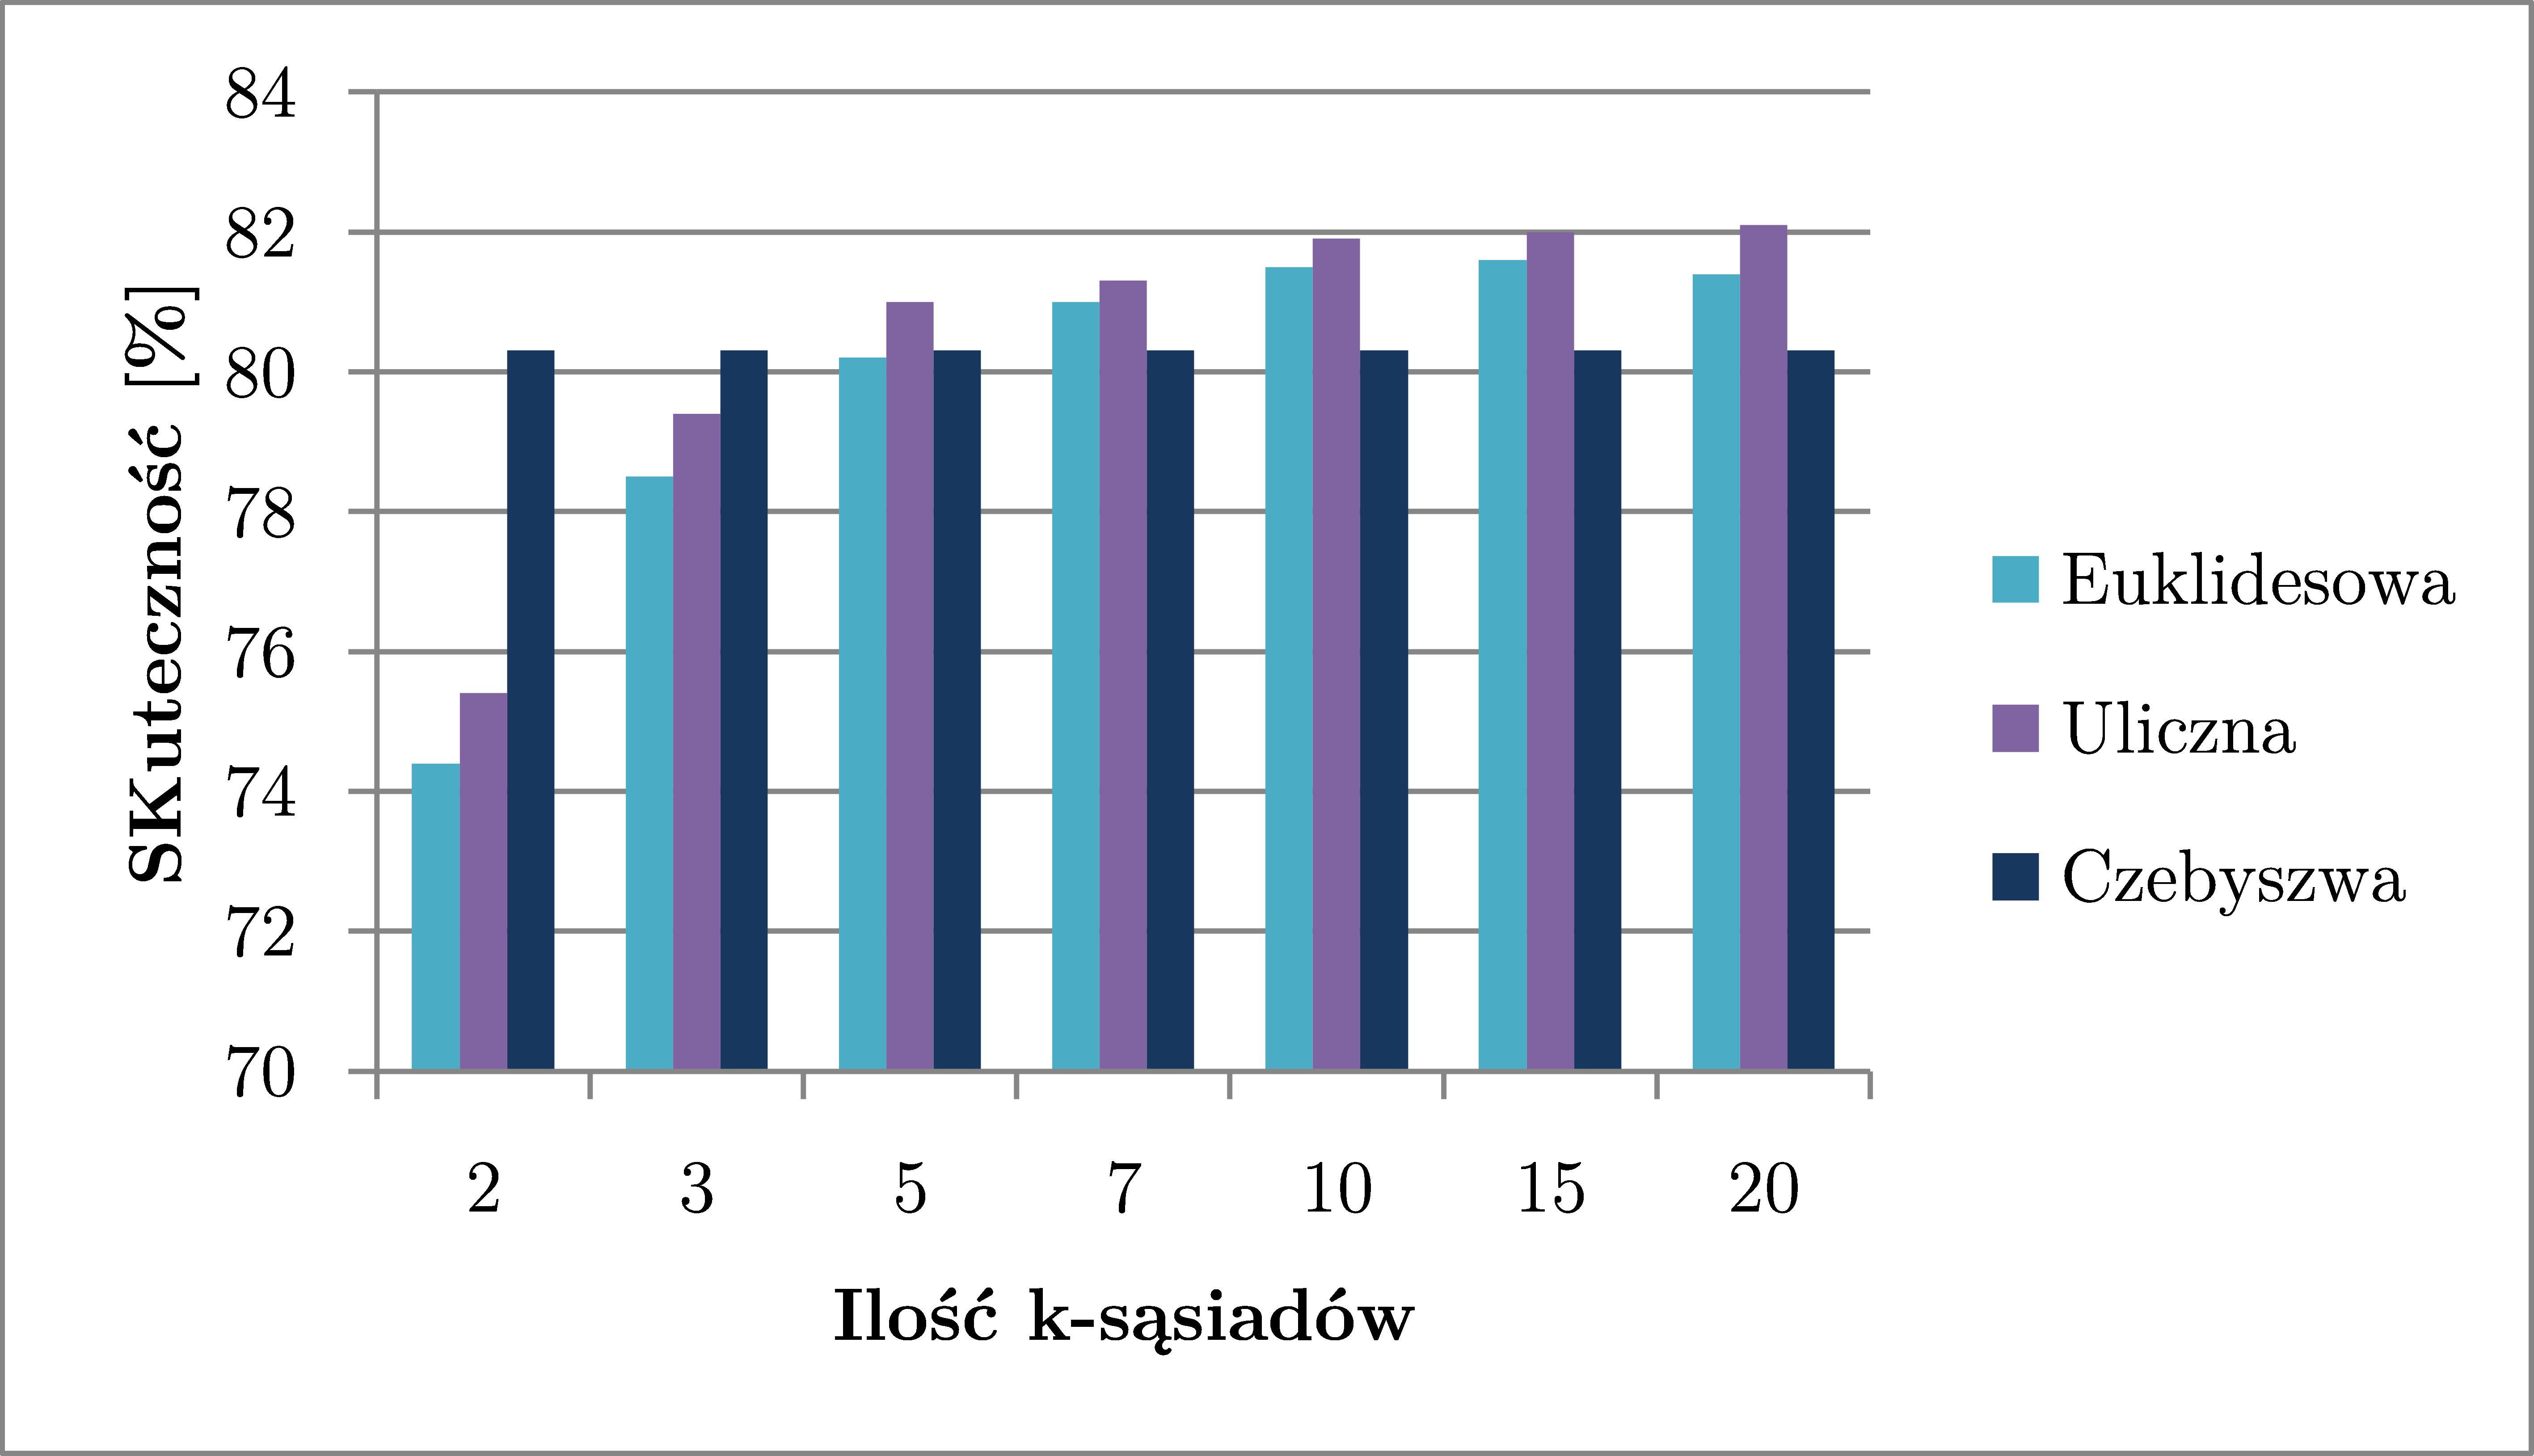
\includegraphics[width=0.8\textwidth]{{Rysunki/TF-places.png}}
	\caption{Dane z Tabel 4-6 dla kategorii places}
\end{figure}

\begin{figure}[H]
	\centering
	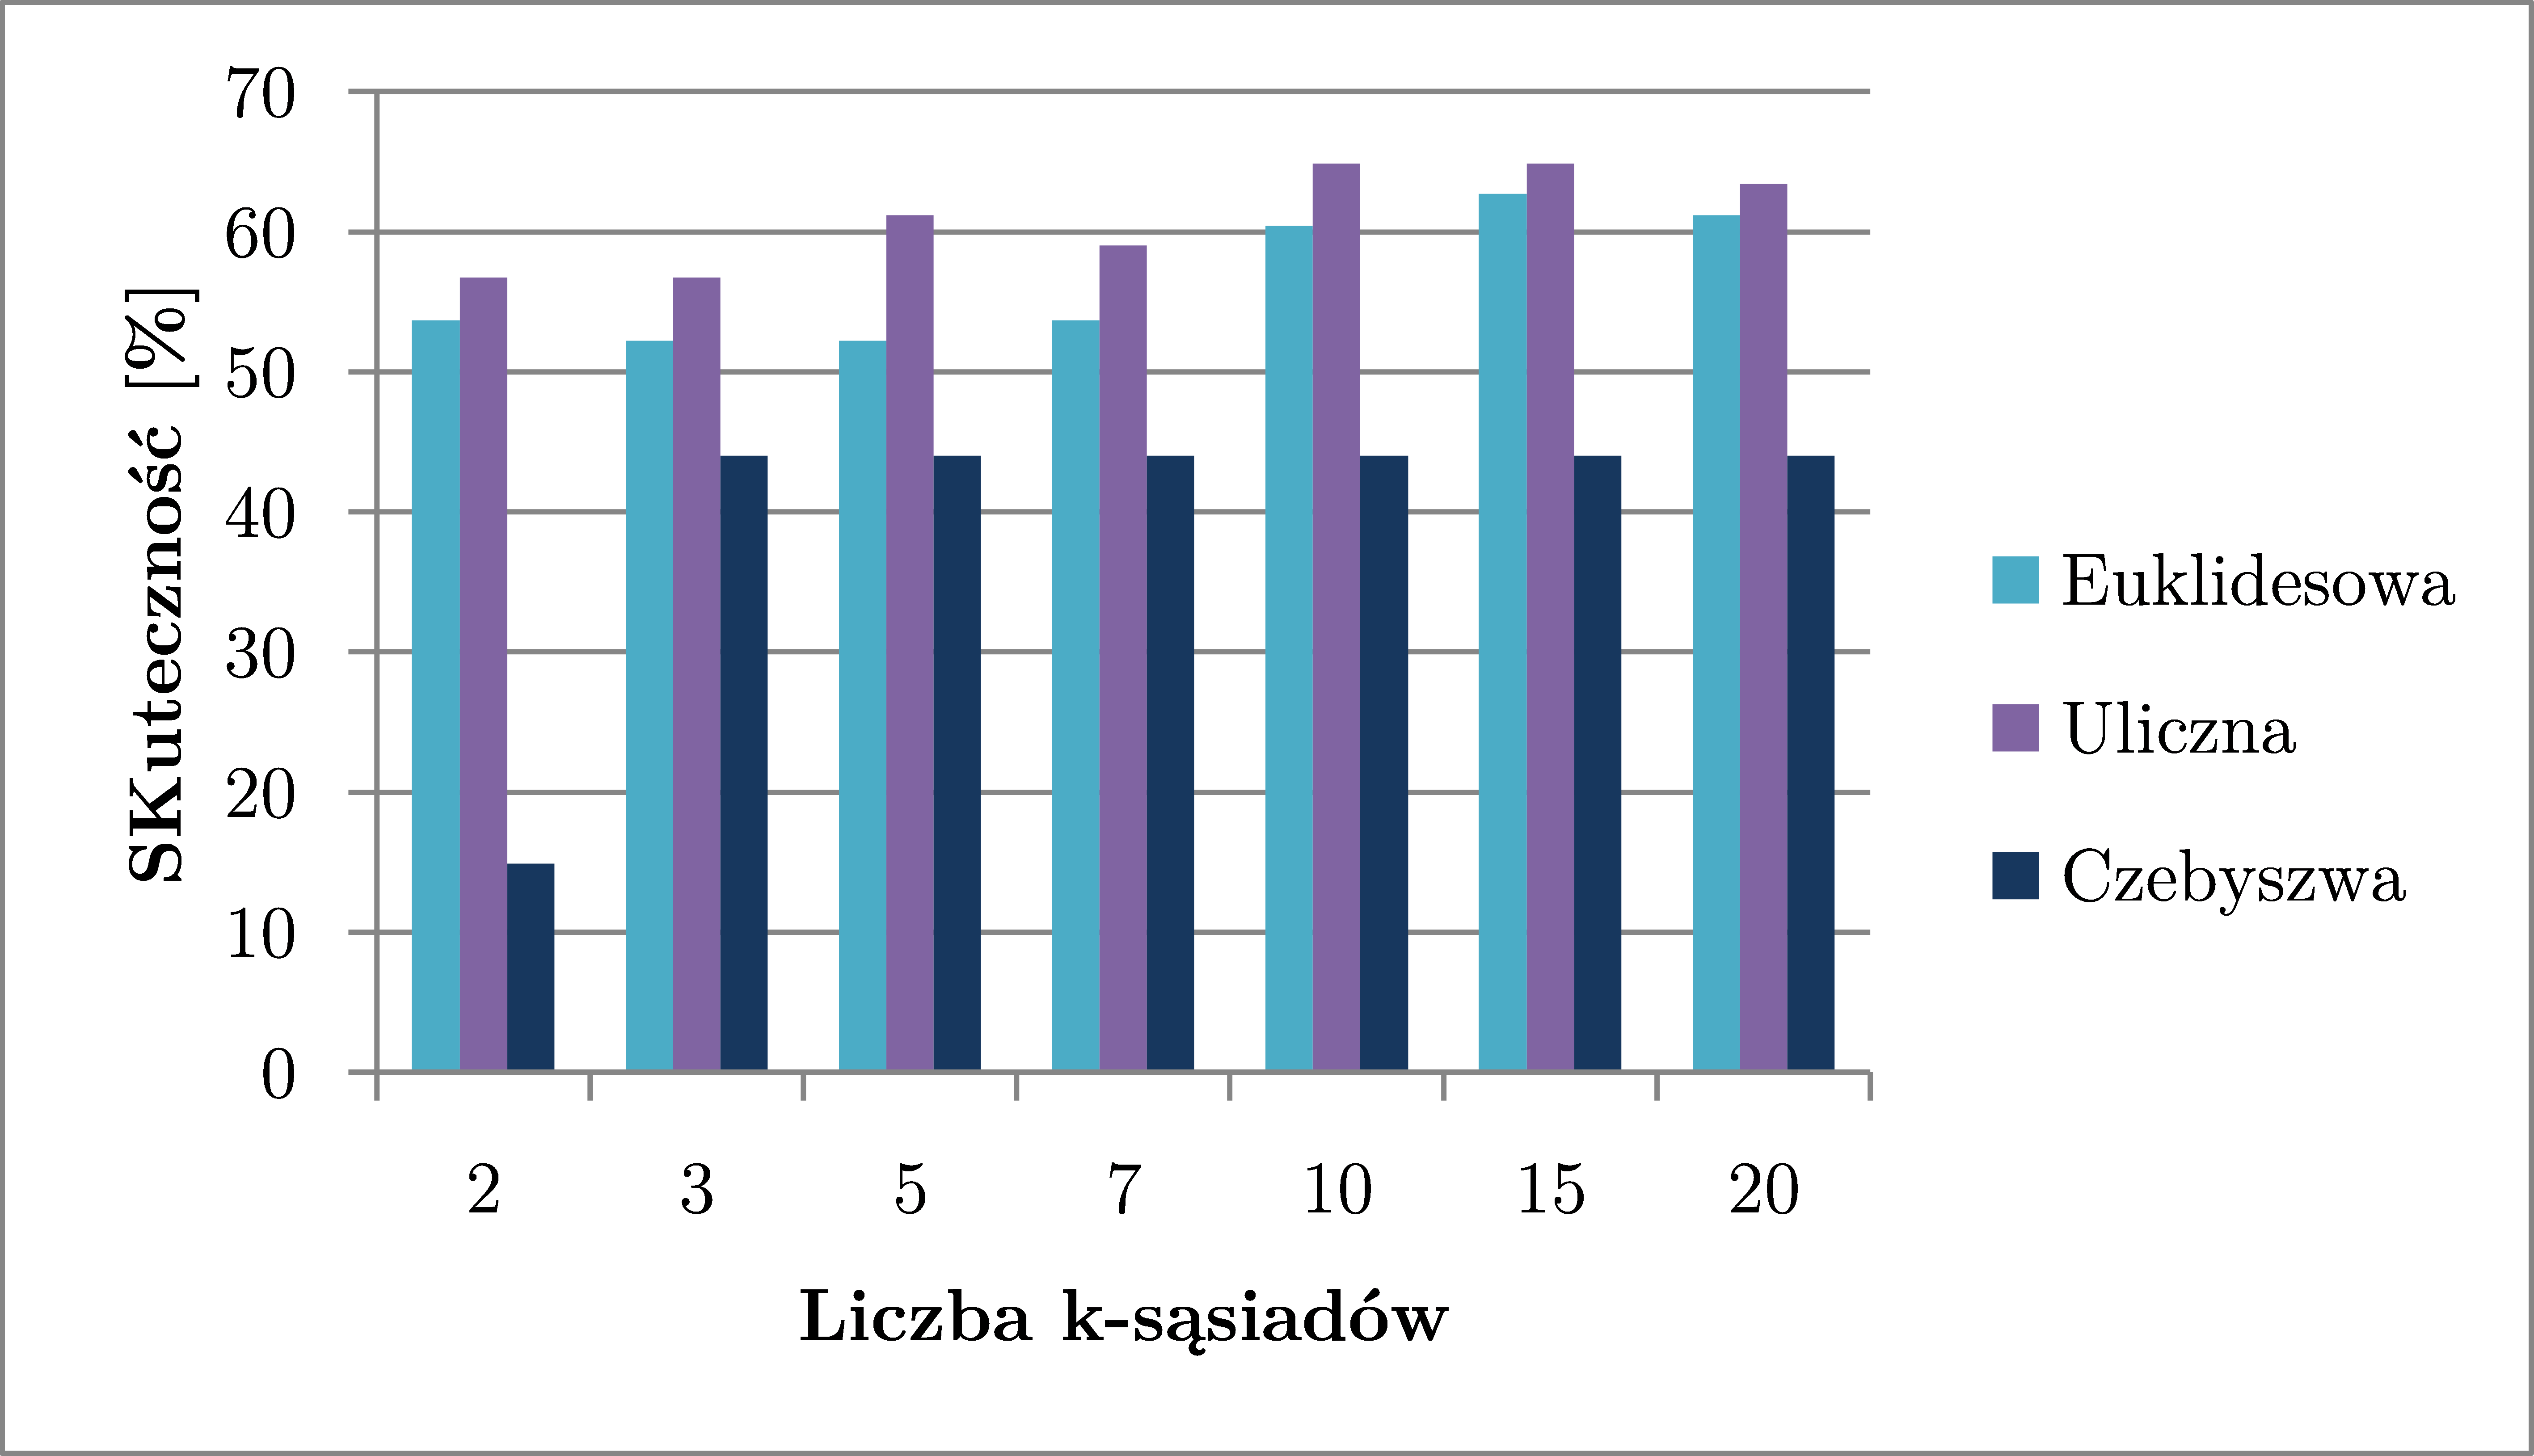
\includegraphics[width=0.8\textwidth]{{Rysunki/TF-topics.png}}
	\caption{Dane z Tabel 4-6 dla kategorii topics}
\end{figure}

\begin{figure}[H]
	\centering
	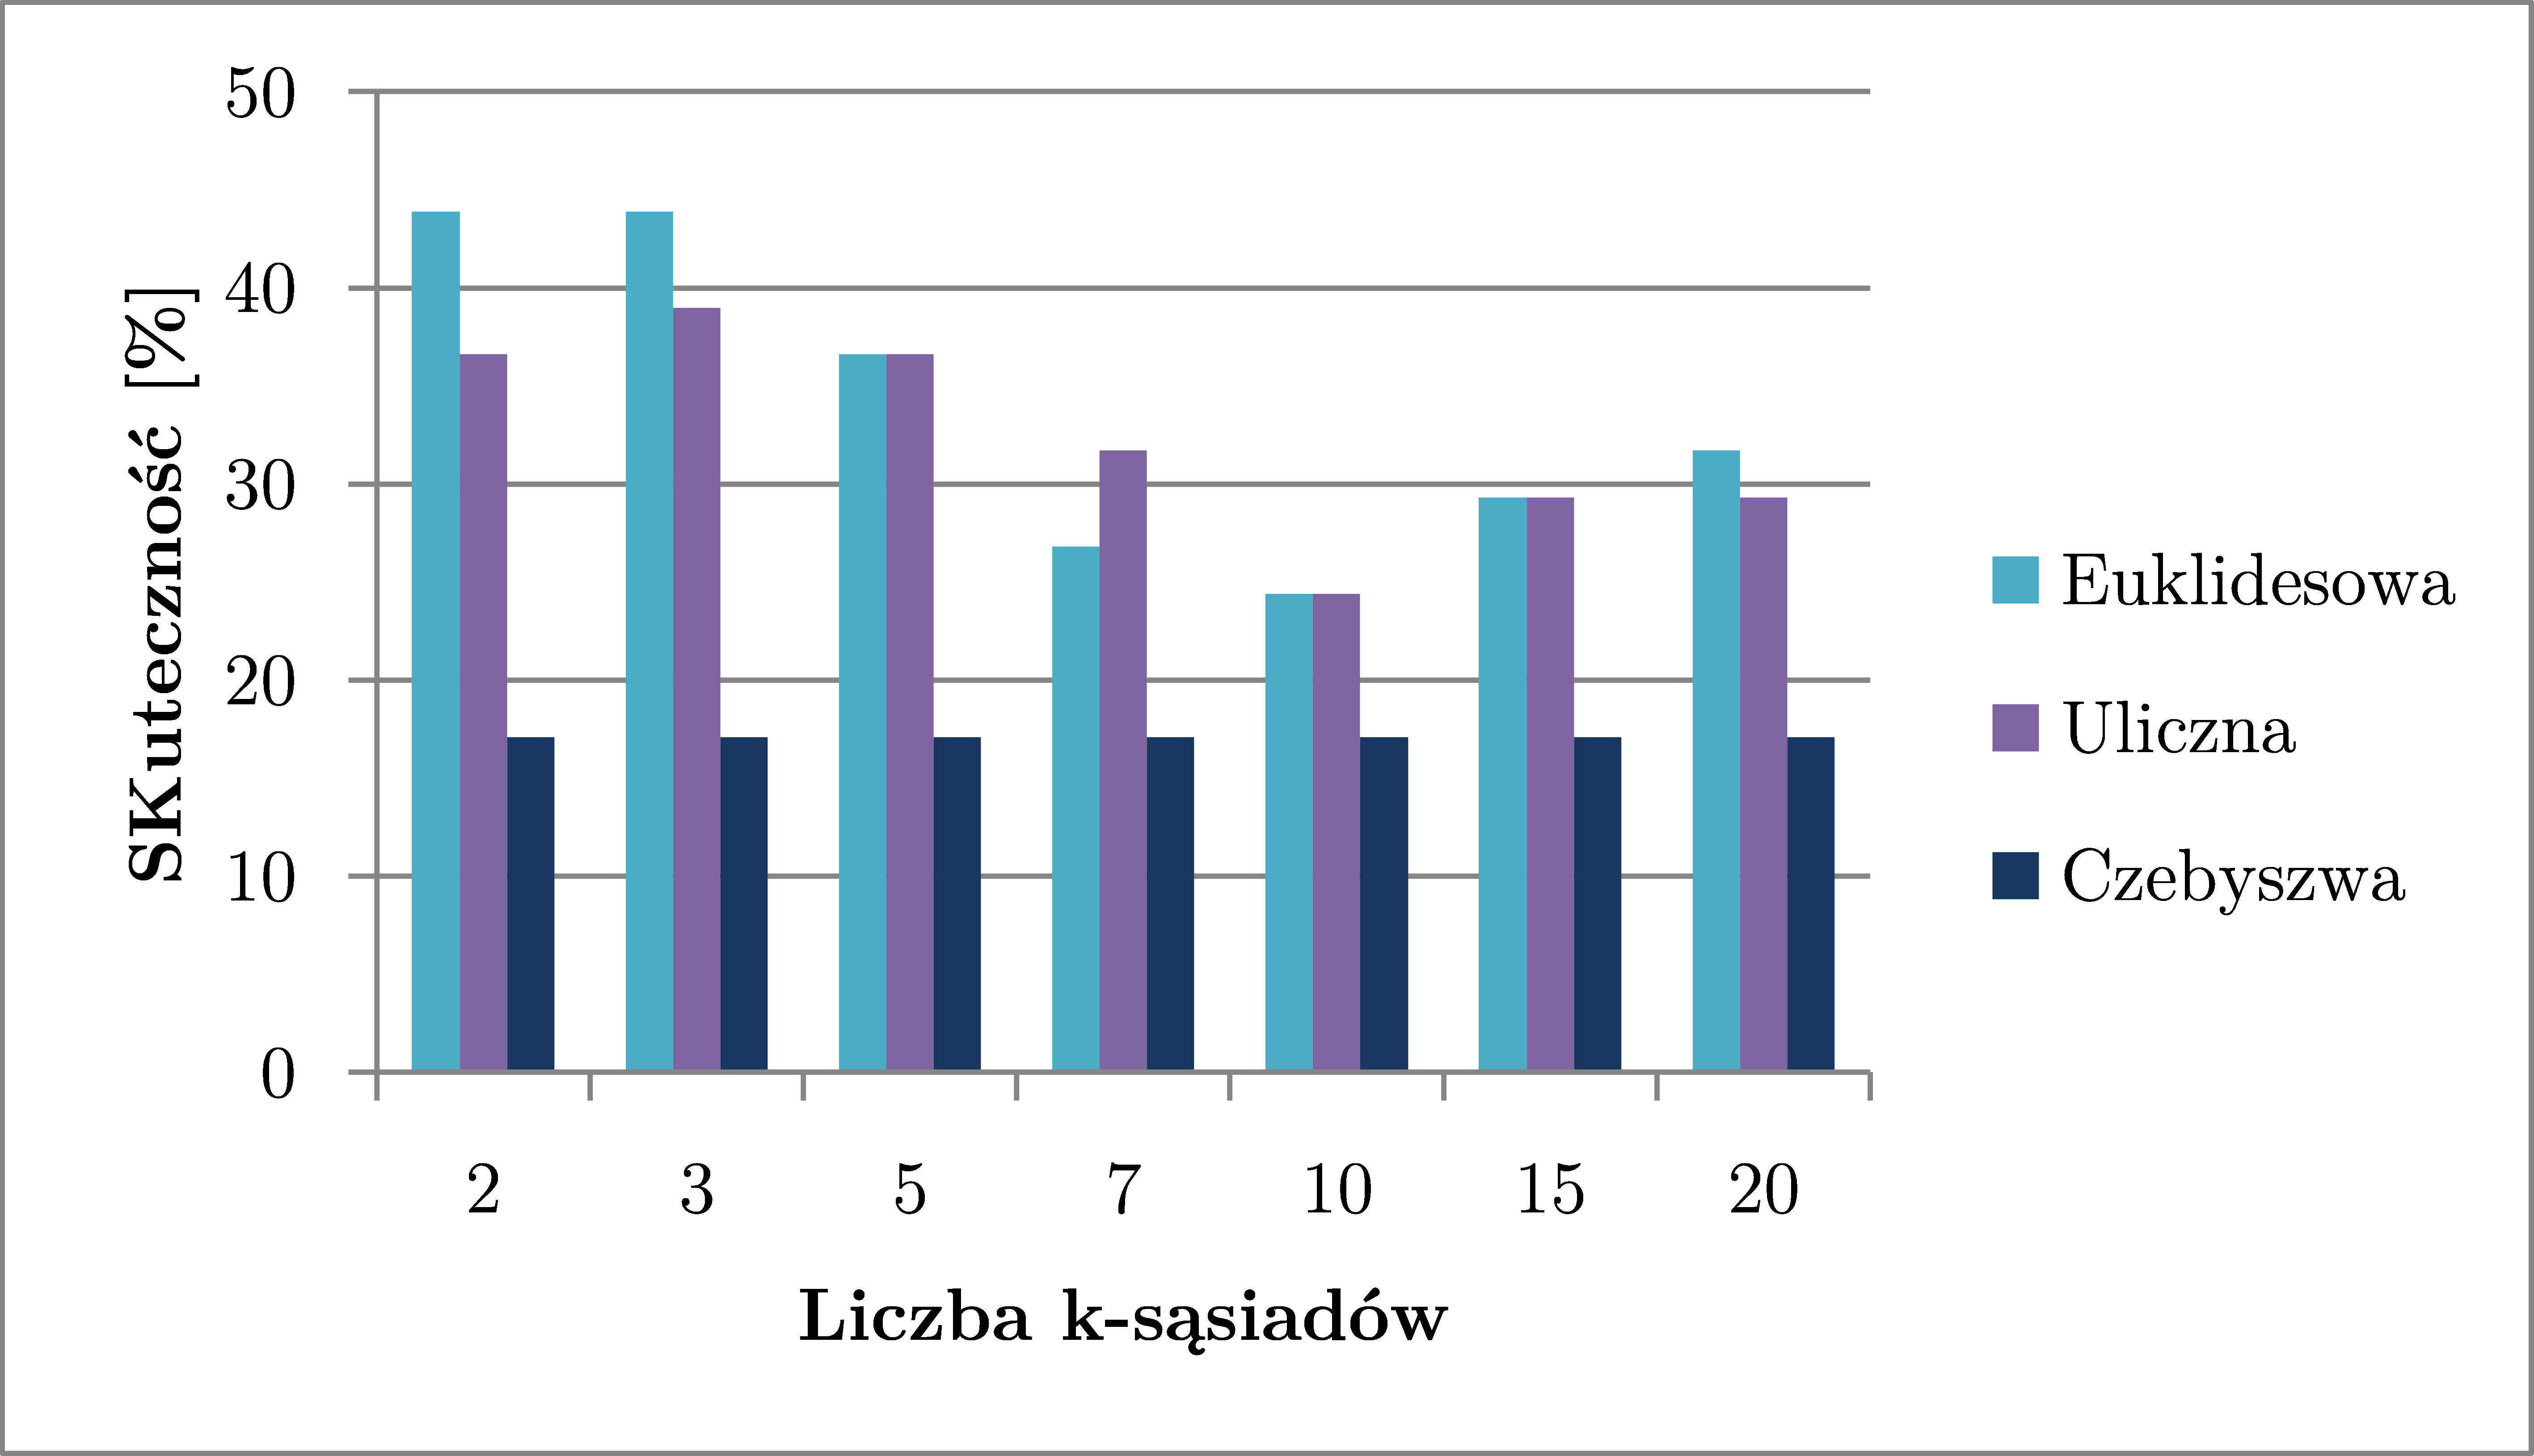
\includegraphics[width=0.8\textwidth]{{Rysunki/TF-authors.png}}
	\caption{Dane z Tabel 4-6 dla kategorii authors (własne teksty)}
\end{figure}

\section{Dyskusja}
	Po przeprowadzonych badaniach jesteśmy w stanie zauważyć, iż metryka uliczna charakteryzuje się największą skutecznością w przypadku pierwszego, jak i drugiego sposobu ekstrakcji cech. Niewiele mniejszą skuteczność wykazuje metryka Euklidesowa. Z kolei, najmniejszą skuteczność reprezentuje metryka Czebyszewa. W przeciwieństwo do dwóch pozostałych metryk, zmiana ilości k sąsiadów nie wpływała lub wpływała nieznacząco na liczbę dopasowanych dokumentów. \newline
	Niska liczba liczba k-sąsiadów (od 2 do 5) zazwyczaj oraz bardzo wysoka ( 20) zazwyczaj negatywnie wpływały na skuteczność. Optymalna liczba sąsiadów do dokonania klasyfikacji w przypadku algorytmu k-nn wynosi 10 w przypadku ekstrakcji metodą term frequency oraz 7 w przypadku ekstrakcji inverse document frequency. \newline
	Dwie użyte przez nas metody ekstrakcji cech wykazują bardzo podobną skuteczność - inverse document frequency nieznacznie przewyższa term frequency. Może to wynikać z faktu, iż IDF przeszukuje wszystkie dokumenty, a TF tylko jeden.  \newline
	
	
\section{Wnioski}
	

\begin{thebibliography}{}
\bibitem{adam}
Methods for the linguistic summarization of data - aplications of fuzzy sets and their extensions, Adam Niewiadomski, Akademicka Oficyna Wydawnicza EXIT, Warszawa 2008
1. http://home.agh.edu.pl/~horzyk/lectures/miw/KNN.pdf
\bibitem{Stop Lista}
https://github.com/hklemp/dotnet-stop-words
\bibitem{Stemizacja}
http://snowball.tartarus.org/algorithms/english/stemmer.html
\end{thebibliography}
\end{document}
